\documentclass[Main]{subfiles}

\begin{document}
\section{Results and Discussion}
This project have ended with the function miniproject(t\_errors, errorloc) in MatLab which runs the meggitt decoder.
It will return 1 if the messages has been decoded the correct code word otherwise 0.
It takes the parameters t\_errors, which is the number of errors which should be added to the message and errorloc which is the location of the errors.
If errorloc is not used the error is added randomly.

Some screen dumps form MatLab calling the miniproject function will be discussed.
the result form calling the function with indicating one error is shown in Figure \ref{fig:result-1-errors}.
It can be seen that the codeword has been decoded successfully.
Furthermore it shows the interested vectors and the tag telling what decoding it has done. 

\begin{figure}[h!]
\centering
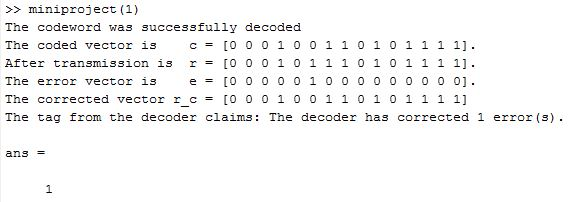
\includegraphics[width=0.7\linewidth]{./Picture/result-1-errors}
\caption{Meggitt decode run with one error, no location}
\label{fig:result-1-errors}
\end{figure}

The Figures \ref{fig:result-2-errors}, \ref{fig:result-2-errors-location} and \ref{fig:result-3-errors} shows the result with other inputs.
In Figure \ref{fig:result-3-errors} it is seen that it is possible to detect there is more errors than 2 but it is not able to correct it. 

\begin{figure}[h!]
\centering
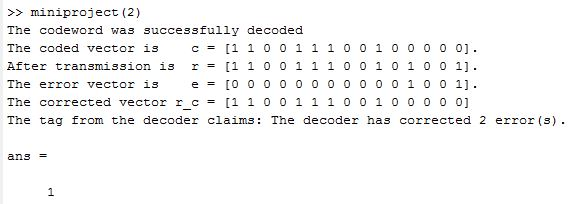
\includegraphics[width=0.7\linewidth]{./Picture/result-2-errors}
\caption{Meggitt decoder run with two errors, no location}
\label{fig:result-2-errors}
\end{figure}

\begin{figure}[h!]
\centering
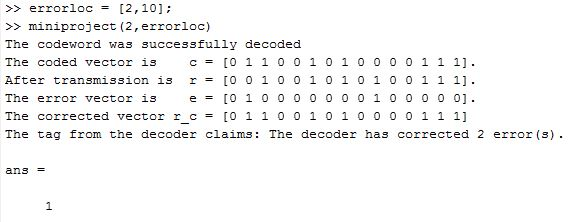
\includegraphics[width=0.7\linewidth]{./Picture/result-2-errors-location}
\caption{Meggit decoder run with 2 errors, with location}
\label{fig:result-2-errors-location}
\end{figure}

\begin{figure}[h!]
\centering
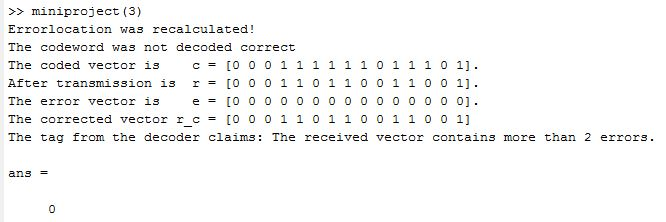
\includegraphics[width=0.7\linewidth]{./Picture/result-3-errors}
\caption{Meggitt decoder run with 3 errors, no location}
\label{fig:result-3-errors}
\end{figure}





%(Giv et input til encoderen --> bliver til)

%(Giv et input til decoderen --> bliver til)
The Meggitt decoder can be tested with the script in \codeTitle \ref{lst:MeggitTest}.
The wanted encoder should return $v(x)$ but has an error, $r(x)$, which must be decoded.
If the value from $isequal$ returns '1' the output is the same as $v(x)$.

\begin{lstlisting}[caption=Meggitt test script, style=Code-Matlab, label=lst:MeggitTest]
%Meggitt decoder
clc, clear

%v(x) - wanted value
v = [1 0 0 1 0 1 1];

%r(x) - v(x) with an error
r = [1 0 0 1 0 0 1];

res = Meggitt(r)

Equal = isequal(v, res)
\end{lstlisting}

$res = [1 0 0 1 0 1 1]$
\\
\\
$Equal = 1 $
(Fejlretning, hvor mange fejl kan vi rette?)\\
Snak om at ved indføring af 3 fejl er der risiko for at det kan blive til et codeword med 2 fejl hvilket vi er i stand til at rette og derfor vi nogle gange får et valid codeword når vi har indført 3 fejl. Dette skylde at vi har en $d_{min}=5$

\end{document}
